
\section{\label{app:gravity} Modifications for a $1/r^2$ Plane-Parallel Basestate}

In the plane parallel assumption, we model a layer of thickness
$\Delta R$ a distance $R_\mathrm{base}$ from the center of a star,
under the assumption the $\Delta R \ll R_\mathrm{base}$.  In this
assumption, we can neglect the curvature of the atmosphere.  Here, we 
extend that basic assumption to allow for the gravitational acceleration
to still fall off as $1/r^2$ as we move outward in the envelope.  We assume
that the mass of the envelope is insignificant, and that only the mass of 
the underlying star contributes to the gravitational acceleration.

\subsection{Constraint Equation}

We begin with the $w_0$ constraint equation (derived elsewhere), including the volume-discrepancy term:
\begin{equation}
\nabla \cdot  ({w_0 \er}) = \bar{S} - \frac{1}{\gammabar p_0} \psi - \frac{f}{\gammabar p_0} \frac{p_0 - \overline{{p_0}_\mathrm{EOS}}}{\dt}
\end{equation}
where
\[ \psi = \frac{D_0 p_0}{D t} = \frac{\partial p_0}{\partial t} + w_0 \frac{\partial p_0}{\partial t}. \]
In Cartesian geometry, the divergence on the left hand side is simply $\partial
w_0 / \partial r$.
Let us now define $\ow$ and $\dw$ such that
\[ w_0 = \ow + \dw \]
We take $\ow$ to satisfy
\begin{equation}
\frac{\partial \ow}{\partial r} = \bar{S} - \frac{f}{\gammabar p_0} \frac{p_0 - \overline{{p_0}_\mathrm{EOS}}}{\dt} ,
\end{equation}
leaving the equation
\begin{equation}
\frac{\partial \dw}{\partial r} = - \frac{1}{\gammabar p_0} \left ({ \frac{\partial p_0}{\partial t} + w_0 \frac{\partial p_0}{\partial r}} \right ).
\end{equation}
%
If we multiply by $\gammabar p_0$, differentiate by r, then switch the order of $\partial
t$ and $\partial r$ where they appear in the same term, we get
\begin{equation}
\frac{\partial}{\partial r} \left[ \gammabar p_0 \frac{\partial \delta w_0}{\partial r} \right] =
   - \frac{\partial}{\partial t} \frac{\partial p_0}{\partial r} -  \frac{\partial}{\partial r} \left (w_0 \frac{\partial p_0}{\partial r} \right) .
\end{equation}
%
We then substitute in the equation of hydrostatic equilibrium:
\[ \frac{\partial p_0}{\partial r} = -\rho_0 g \quad\quad \mbox{where} \quad\quad
   g = \frac{G m}{r^2}. \]
We will assume that the mass of the atmosphere is negligible relative to the
mass of the core, which is outside of the simulation domain.  This simplifies
the equation by allowing us to assume that $m$, the enclosed mass, is constant.
So we now have
\begin{equation}
\frac{\partial}{\partial r} \left[ \gammabar p_0 \frac{\partial}{\partial r}{({\delta w_0})} \right]
   = \frac{\partial}{\partial t}{({\rho_0 g}}) + \frac{\partial}{\partial r}{({w_0 \rho_0 g})}
   = \rho_0 \left ({\frac{\partial}{\partial t}{g} + w_0 \frac{\partial}{\partial r}{g}} \right )
         + g \left ({\frac{\partial}{\partial t}{\rho_0} + \frac{\partial}{\partial r}{({w_0 \rho_0})}} \right ).
\end{equation}

We now recall Equation~29 from Paper III:
\[ \frac{\partial}{\partial t}{\rho_0} = - \nabla \cdot ({w_0 \rho_0 \er})
                  - \nabla \cdot ({\etarho \er}), \]
which is, in Cartesian geometry,
\begin{equation}
\frac{\partial \rho_0}{\partial t} = - \frac{\partial}{\partial r}{({w_0 \rho_0})}
                  - \frac{\partial \etarho}{\partial r}.
\end{equation}
Substituting this expression yields
\begin{equation}
\frac{\partial}{\partial r}{} \left[ \gammabar p_0 \frac{\partial}{\partial r}{({\delta w_0})} \right]
   = \rho_0 \frac{D_0 g}{D t} + g \left ({- \frac{\partial}{\partial r}{({w_0 \rho_0})} - \frac{\partial \etarho}{\partial r} + \frac{\partial}{\partial r}{({w_0 \rho_0})}} \right)
   = \rho_0 \frac{D_0 g}{D t} - g \frac{\partial \etarho}{\partial r}.
\end{equation}

We then differentiate the gravitational acceleration:
\begin{eqnarray}
\frac{D_0 g}{D t}
   & = & \frac{D_0}{Dt} \left ({\frac{G m}{r^2}} \right ) \nonumber \\
   & = & G m \left ({\frac{\partial}{\partial t}{({r^{-2}})} + w_0 \frac{\partial}{\partial r}{({r^{-2}})}} \right ) \nonumber \\
   & = & - \frac{2 G m w_0}{r^3} \nonumber \\
   & = & - \frac{2 w_0 g}{r}.
\end{eqnarray}
Substituting in this expression gives our final result:
\begin{equation}
\frac{\partial}{\partial r}{} \left[ \gammabar p_0 \frac{\partial}{\partial r}{({\dw})} \right]
   = - \frac{2 w_0 \rho_0 g}{r} - g \frac{\partial \etarho}{\partial r}
\end{equation}

\subsection{Uniform $\dr$ Discretization}

Collecting all of the $\dw$ terms on the left side, our constraint equation
appears as:
\begin{equation}
\frac{\partial}{\partial r} \left [ \gammabar p_0 \frac{\partial \dw}{\partial r} \right ]
 + \frac{2 \rho_0 g \dw}{r} = -\frac{2 \rho_0 g \ow}{r} - g \frac{\partial \etarho}{\partial r}
\end{equation}
%
On a uniform mesh (constant $\dr$, we would discretize this as:
\begin{eqnarray}
\frac{1}{\dr} \left \{ \left [ \gammabar p_0 \frac{\partial \dw}{\partial r} \right ]_j
                     - \left [ \gammabar p_0 \frac{\partial \dw}{\partial r} \right ]_{j-1}
              \right \}
            &+& \left [ \frac{2 \rho_0 g}{r} \dw \right ]_{j-\half} \nonumber \\
            = &-& \left [ \frac{2 \rho_0 g}{r} \ow \right ]_{j-\half}
              - \frac{g_{j-\half}}{\dr} \left [ {\etarho}_j - {\etarho}_{j-1} \right ]
\end{eqnarray}
Expanding the $\partial \dw / \partial r$ terms, we have:
\begin{eqnarray}
\frac{1}{(\dr)^2} \left \{ \left [ (\gammabar p_0)_j
                               \left ({\dw}_{j+\half} - {\dw}_{j-\half} \right ) \right ]
                      \right . &-& \left . \left [ (\gammabar p_0)_{j-1}
                               \left ({\dw}_{j-\half} - {\dw}_{j-\thalf} \right ) \right ]
              \right \}
            + \left [ \frac{2 \rho_0 g}{r} \dw \right ]_{j-\half} \nonumber \\
            = &-& \left [ \frac{2 \rho_0 g}{r} \ow \right ]_{j-\half}
              - \frac{g_{j-\half}}{\dr} \left [ {\etarho}_j - {\etarho}_{j-1} \right ]
\end{eqnarray}
As with the spherical case (multilevel paper, appendix B), we write this in the form:
\begin{equation}
A_j (\dw)_{j-\thalf} + B_j (\dw)_{j-\myhalf} + C_j (\dw)_{j+\myhalf} = F_j,
\end{equation}
then:
\begin{eqnarray}
A_j &=& \frac{1}{\dr^2} \left( {\gammabar p_0}\right)_{j-1}, \\
B_j &=& -\frac{1}{\dr^2} \left[ \left( {\gammabar p_0}\right)_{j}  + \left( {\gammabar p_0}\right)_{j-1} \right] +  \frac{2}{r_{j-\myhalf}} \left (\rho_0 g \right )_{j-\half}  , \\
C_j &=& \frac{1}{\dr^2} \left( {\gammabar p_0}\right)_{j}  , \\
F_j &=&  -\frac{2}{r_{j-\myhalf}} (\rho_0 g)_{j-\half}   (\ow)_{j-\half} - \frac{g_{j-\half}}{\dr} \left[ \left( \etarho \right)_{j} - \left( \etarho \right)_{j-1} \right] 
\end{eqnarray}


\subsection{Non-Uniform $\dr$ Discretization}

\begin{figure}[h]
\centering
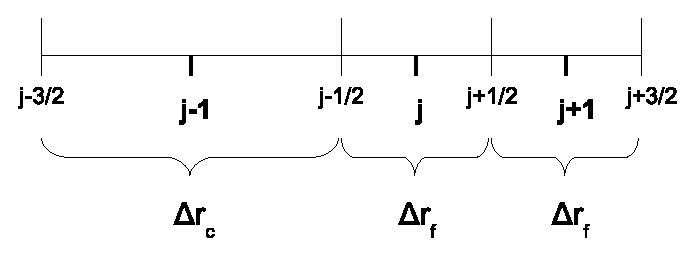
\includegraphics[width=4in]{\planeinvsqfigpath/grid2}
\end{figure}

Consider the above non-uniform grid spacing,
where $\dr_c = 2 \dr_f$.  Here, the discretization of the Laplacian-like term is more complex.
We want to compute
\begin{equation}
\frac{\partial}{\partial r} \left [ \gammabar p_0 \frac{\partial \dw}{\partial r} \right ]_{j-\half}
\end{equation}
This is to be centered at $j-\half$, which we accomplish by averaging the two fine grids and then
differencing:
\begin{equation}
\frac{\partial}{\partial r} \left [ \gammabar p_0 \frac{\partial \dw}{\partial r} \right ]_{j-\half} =
\frac{1}{\dr_c} \left \{ \frac{1}{2} \left [
      \left ( \gammabar p_0 \frac{\partial \dw}{\partial r} \right )_{j+1} +
      \left ( \gammabar p_0 \frac{\partial \dw}{\partial r} \right )_{j} \right ]
   - \left ( \gammabar p_0 \frac{\partial \dw}{\partial r} \right )_{j-1} 
\right \}
\end{equation}
Expanding the $\partial \dw / \partial r$ terms results in a equation depending on $\dw$ at
4 different edge locations---this no longer fits into the tri-diagonal format used in the
uniform grid case.  In detail, it becomes:
\begin{eqnarray}
\frac{\partial}{\partial r} \left [ \gammabar p_0 \frac{\partial \dw}{\partial r} \right ]_{j-\half} &=& 
\frac{1}{\dr_c} \left \{  \frac{1}{2} \left [
      \left ( \gammabar p_0 \right )_{j+1} \frac{(\dw)_{j+\thalf} - (\dw)_{j+\half}}{\dr_f} +
      \left ( \gammabar p_0 \right )_{j}   \frac{(\dw)_{j+\half} - (\dw)_{j-\half}}{\dr_f}  \right ] \right .  \nonumber \\
&& \qquad \left .  - \left ( \gammabar p_0 \right )_{j-1} \frac{(\dw)_{j-\half} - (\dw)_{j-\thalf}}{\dr_c}  
\right \}
\end{eqnarray}
which has terms proportional to $(\dw)_{j-\thalf}$, $(\dw)_{j-\half}$, $(\dw)_{j+\half}$, and $(\dw)_{j+\thalf}$


\subsection{Boundary Conditions}

Together with the assumption that the mass of the envelope does not
contribute to the gravitational acceleration, we assume that as we move
a fluid element in the atmosphere, it does not drive a velocity at the very 
base of the layer.  Therefore, we take $w_0(r_\mathrm{base}) = 0$.



